\documentclass[a4paper]{article}
\usepackage{../mystyle}

\begin{document}

\includepdf[pages={1}]{../titul/titul.pdf}

\tableofcontents

\newpage

\section{Описание предметной области}

\subsection{Формулировка задания}
Спроектировать базу данных для проведения Единого Государственного
экзамена, проводящегося ежегодно в школах разных городов Российской
Федерации. База данных должна содержать информацию о студентах, школах и
учителях, а также отражать ежегодные данные по сдаваемым предметам,
составленное расписание и полученные учениками результаты.

\subsection{Конкретизация предметной области}
Необходимо создать систему, отражающую информацию о проведении и
результатах экзаменов по всей стране. По каждому предмету есть ежегодная
информация, так как Министерство образования ежегодно вносит коррективы в тот
или иной экзамен. База данных должна отражать точное расписание экзаменов по
всем городам каждый год, а также результаты конкретного ученика по всем выбранным им предметам.

\subsection{Пользователи системы}
Основными пользователями системы являются:
\begin{itemize}
      \item \textbf{Администраторы школ} - управляют данными учебных заведений, аудиториями, расписанием экзаменов
      \item \textbf{Преподаватели} - ведут учет предметов, заданий, результатов экзаменов
      \item \textbf{Учащиеся} - просматривают расписание экзаменов, свои результаты
      \item \textbf{Экзаменационная комиссия} - вносит результаты экзаменов, проверяет работы
      \item \textbf{Технические специалисты} - обслуживают систему, обеспечивают целостность данных
\end{itemize}

\subsection{Сроки хранения информации}
\begin{itemize}
      \item \textbf{Персональные данные учащихся} - хранятся до 5 лет после окончания обучения
      \item \textbf{Результаты экзаменов (ExamResult)} - хранятся постоянно в архиве
      \item \textbf{Расписание экзаменов (Exam)} - хранится 3 года после даты проведения
      \item \textbf{Учебные задания (Task)} - хранятся 5 лет для возможного апелллирования
      \item \textbf{Справочная информация} (школы, адреса, предметы) - хранится постоянно
\end{itemize}

\subsection{События, изменяющие состояние базы данных}
Критические события системы:
\begin{itemize}
      \item Добавление/изменение расписания экзаменов (сущность Exam)
      \item Регистрация учащегося на экзамен (отношение go\_to)
      \item Внесение результатов экзамена (сущность ExamResult)
      \item Назначение преподавателя на предмет (отношение lead)
      \item Изменение состава экзаменационной комиссии (отношение work\_at)
      \item Подача апелляции (изменение статуса в ExamResult)
      \item Обновление учебных заданий (сущность Task)
\end{itemize}

\subsection{Основные запросы к базе данных (на естественном языке)}
\begin{itemize}
      \item Получить расписание всех экзаменов для указанной школы на заданную дату
      \item Найти всех учащихся, сдающих конкретный предмет в указанный период
      \item Показать средний балл по предмету для выбранной школы
      \item Получить список всех аудиторий, занятых в определенный день
      \item Найти всех преподавателей, ведущих указанный предмет
      \item Получить историю экзаменов конкретного учащегося с результатами
      \item Показать распределение оценок по конкретному экзамену
      \item Найти всех учащихся, проживающих в указанном городе/районе
      \item Получить список заданий для конкретного варианта экзамена
      \item Показать статистику сдачи экзаменов по школам за указанный период
\end{itemize}

\section{Концептуально-информационная модель предметной области}

\subsection{Er-диаграмма модели}
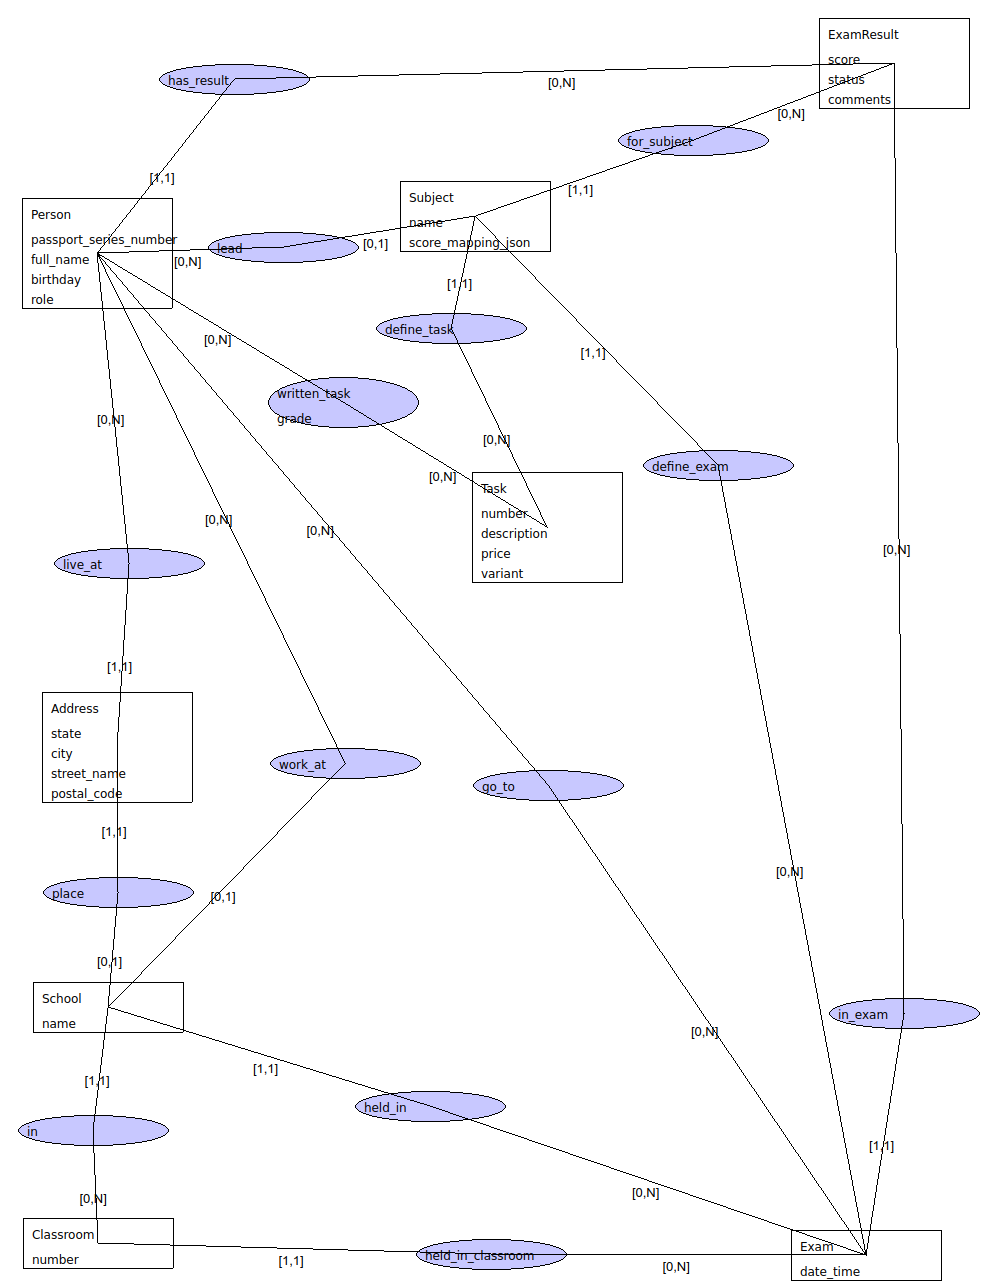
\includegraphics[width=14cm]{data/er.png}

\subsection{Оценка мощностных характеристик сущностей и связей}

\subsubsection{Оценка мощностных характеристик сущностей}
\begin{itemize}
      \item \textbf{Сущность Address}:
            \begin{itemize}
                  \item Ожидаемое количество: 251,000 \newline
                        Формула: $1000_{\text{школ}} + 500000_{\text{учеников}} + 150000_{\text{учителей}}$
            \end{itemize}

      \item \textbf{Сущность School}:
            \begin{itemize}
                  \item Ожидаемое количество: 1,000
            \end{itemize}

      \item \textbf{Сущность Man}:
            \begin{itemize}
                  \item Ожидаемое количество: 650,000 \newline
                        Формула: $100000_{\text{учеников}} \times 5_{\text{лет}} + 150000_{\text{учителей}}$
            \end{itemize}

      \item \textbf{Сущность Subject}:
            \begin{itemize}
                  \item Ожидаемое количество: 16
            \end{itemize}

      \item \textbf{Сущность Exam}:
            \begin{itemize}
                  \item Ожидаемое количество: 8,000 \newline
                        Формула: $16_{\text{предметов}} \times 100_{\text{школ/год}} \times 5_{\text{лет}}$
            \end{itemize}

      \item \textbf{Сущность ExamResult}:
            \begin{itemize}
                  \item Ожидаемое количество: 1,500,000 \newline
                        Формула: $100000_{\text{учеников/год}} \times 3_{\text{предмета}} \times 5_{\text{лет}}$
            \end{itemize}

      \item \textbf{Сущность Task}:
            \begin{itemize}
                  \item Ожидаемое количество: 48,000 \newline
                        Формула: $16_{\text{предметов}} \times 30_{\text{заданий}} \times 5_{\text{лет}} \times 20_{\text{вариантов}}$
            \end{itemize}

      \item \textbf{Сущность Classroom}:
            \begin{itemize}
                  \item Ожидаемое количество: 20,000 \newline
                        Формула: $20_{\text{аудиторий/школу}} \times 1000_{\text{школ}}$
            \end{itemize}
\end{itemize}

\subsubsection{Оценка мощностных характеристик связей}
\begin{itemize}
      \item \textbf{written\_task}:
            \begin{itemize}
                  \item Ожидаемое количество: 3,000,000 \newline
                        Формула: $1.5\text{M}_{\text{результатов}} \times 30_{\text{заданий}}$
            \end{itemize}

      \item \textbf{go\_to}:
            \begin{itemize}
                  \item Ожидаемое количество: 1,500,000 \newline
                        Формула: ExamResult
            \end{itemize}

      \item \textbf{has\_result}:
            \begin{itemize}
                  \item Ожидаемое количество: 1,500,000 \newline
                        Формула: ExamResult
            \end{itemize}

      \item \textbf{live\_at}:
            \begin{itemize}
                  \item Ожидаемое количество: 650,000 \newline
                        Формула: Man
            \end{itemize}

      \item \textbf{work\_at}:
            \begin{itemize}
                  \item Ожидаемое количество: 150,000 \newline
                        Формула: (количество учителей)
            \end{itemize}
\end{itemize}

\section{Концептуальное проектирование}

\subsection{Принятые проектные соглашения}

В проекте базы данных для системы "Расписание и сдача ЕГЭ" приняты следующие соглашения:

\begin{itemize}
      \item \textbf{Именование объектов}:
            \begin{itemize}
                  \item Таблицы - в единственном числе (School, Man, Subject)
                  \item Поля - в snake\_case (passport\_series\_number, street\_name)
            \end{itemize}

      \item \textbf{Типы данных}:
            \begin{itemize}
                  \item Для персональных данных - VARCHAR с ограничением длины
                  \item Даты - тип DATE или TIMESTAMP
                  \item JSON-данные (score\_mapping\_json) - тип JSONB
            \end{itemize}

      \item \textbf{Нормализация}:
            \begin{itemize}
                  \item База данных приведена к 3НФ
            \end{itemize}

      \item \textbf{Архитектура}:
            \begin{itemize}
                  \item Клиент-серверная архитектура
                  \item Использование хранимых процедур для сложных операций
            \end{itemize}
\end{itemize}

\subsection{Обоснование выбора модели базы данных}

Для системы "Расписание и сдача ЕГЭ" выбрана реляционная модель базы данных по следующим причинам:

\begin{itemize}
      \item \textbf{Структурированность данных}:
            \begin{itemize}
                  \item Четко определенные связи между сущностями
                  \item Жесткая схема данных обеспечивает целостность
            \end{itemize}

      \item \textbf{Транзакционность}:
            \begin{itemize}
                  \item Требуется ACID-совместимость для операций с результатами экзаменов
                  \item Важна согласованность данных при параллельном доступе
            \end{itemize}

      \item \textbf{Масштабируемость}:
            \begin{itemize}
                  \item Предсказуемый рост данных
                  \item Возможность репликации для отчетных серверов
            \end{itemize}

      \item \textbf{Безопасность}:
            \begin{itemize}
                  \item Разграничение доступа на уровне строк (RLS)
                  \item Поддержка шифрования данных
            \end{itemize}
\end{itemize}

\subsection{Используемые в системе кодификаторы}

\begin{itemize}
      \item \textbf{Кодификатор предметов (Subject)}:
            \begin{itemize}
                  \item Цифровой код (например, 01 - Математика, 02 - Физика)
                  \item Соответствует официальным кодам ЕГЭ
            \end{itemize}

      \item \textbf{Кодификатор территорий (Address)}:
            \begin{itemize}
                  \item Код региона
            \end{itemize}

      \item \textbf{Кодификатор статусов экзамена (ExamResult)}:
            \begin{itemize}
                  \item 0 - Зарегистрирован
                  \item 1 - Сдан
                  \item 2 - Не сдан
                  \item 3 - На апелляции
                  \item 4 - Аннулирован
            \end{itemize}
\end{itemize}

\subsection{Концептуальная модель базы данных}
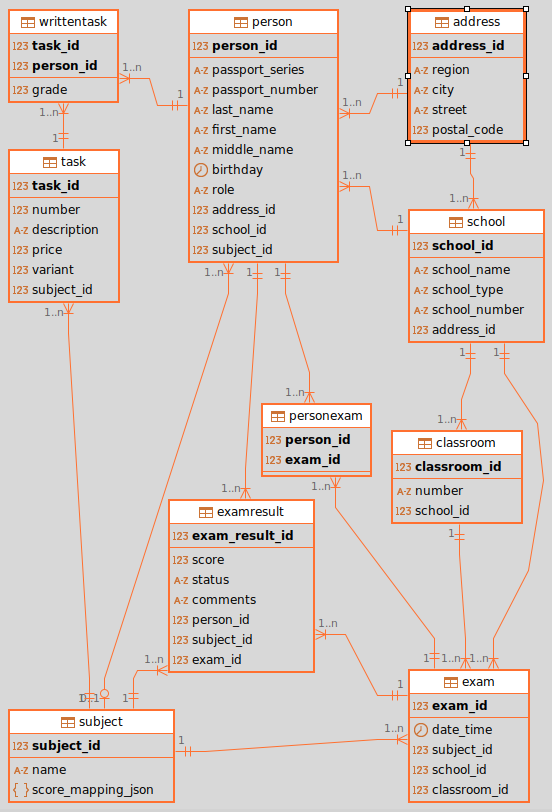
\includegraphics[width=13cm]{data/er_kmdb.png}

\section{Логическое проектирование}

\subsection{Er-диаграмма базы данных (logical)}
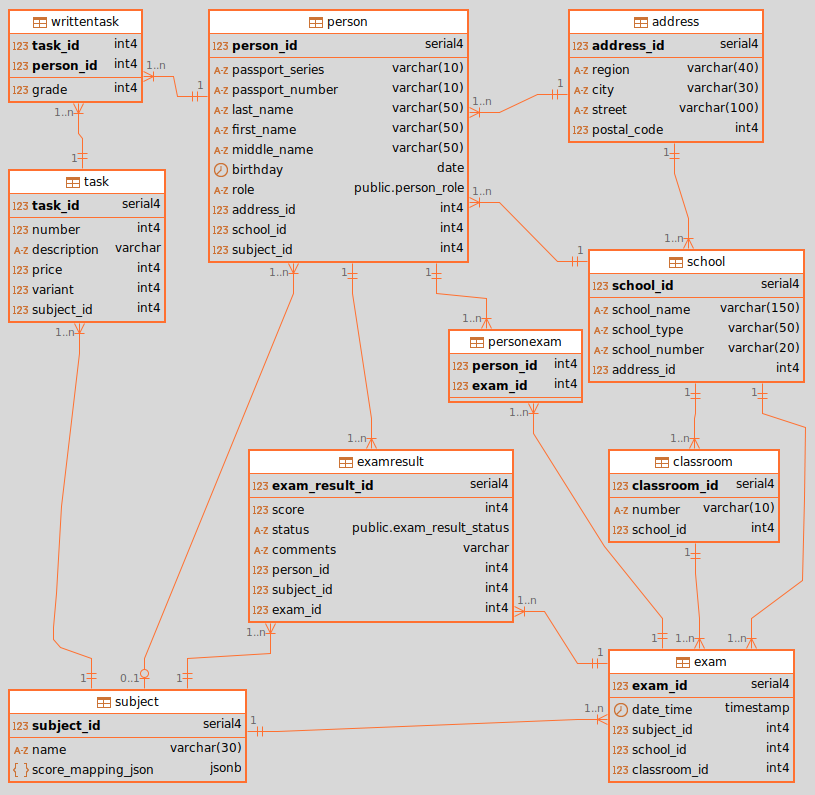
\includegraphics[width=14cm]{data/logical.png}

\subsection{Схемы отношений базы данных (physical)}
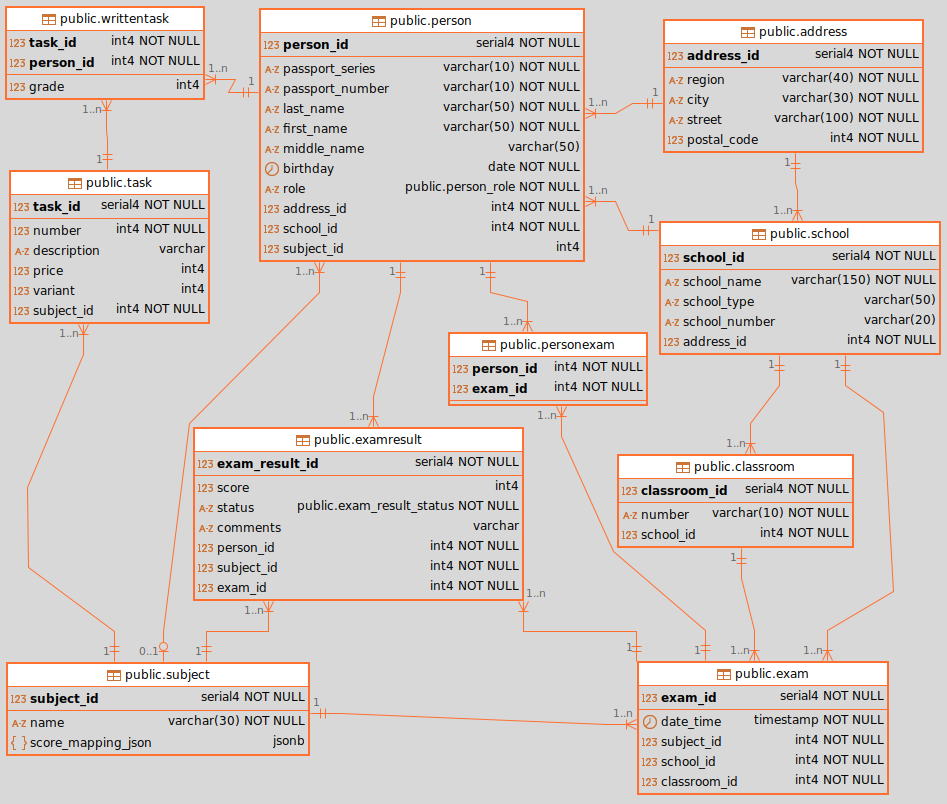
\includegraphics[width=14cm]{data/physical.png}

\subsection{Схема реляционной базы данных}

\renewcommand{\arraystretch}{1.5}
\begin{tabular}{|p{10cm}|p{2cm}|}
      \hline
      Address(\underline{address\_id}, region, city, street, postal\_code)                                                                                            & R1  \\
      \hline
      Subject(\underline{subject\_id}, name, score\_mapping\_json)                                                                                                    & R2  \\
      \hline
      School(\underline{school\_id}, school\_name, school\_type, school\_number, address\_id)                                                                         & R3  \\
      \hline
      Person(\underline{person\_id}, passport\_series, passport\_number, last\_name, first\_name, middle\_name, birthday, role, address\_id, school\_id, subject\_id) & R4  \\
      \hline
      Classroom(\underline{classroom\_id}, number, school\_id)                                                                                                        & R5  \\
      \hline
      Exam(\underline{exam\_id}, date\_time, subject\_id, school\_id, classroom\_id)                                                                                  & R6  \\
      \hline
      Task(\underline{task\_id}, number, description, price, variant, subject\_id)                                                                                    & R7  \\
      \hline
      ExamResult(\underline{exam\_result\_id}, score, status, comments, person\_id, subject\_id, exam\_id)                                                            & R8  \\
      \hline
      PersonExam(\underline{person\_id}, \underline{exam\_id})                                                                                                        & R9  \\
      \hline
      WrittenTask(\underline{task\_id}, \underline{person\_id}, grade)                                                                                                & R10 \\
      \hline
\end{tabular}
\renewcommand{\arraystretch}{1}

\subsection{Схемы основных запросов на реляционной алгебре}

\begin{itemize}
      \item Получить всех учителей, зарегистрированных на экзамен по предмету "Name"
            \begin{lstlisting}[basicstyle=\ttfamily\small, breaklines=true, frame=none, numbers=none]
TeachersMathExam(id) = ((Person[Person.role = 'Teacher' & Person.subject_id = Subject.subject_id] Subject)[Subject.name = 'Name'][Person.person_id = PersonExam.person_id] PersonExam)[Person.person_id]
\end{lstlisting}

      \item Найти всех школьников, не зарегистрированных ни на один экзамен
            \begin{lstlisting}[basicstyle=\ttfamily\small, breaklines=true, frame=none, numbers=none]
UnregisteredStudents(id) = (Person[Person.role = 'SchoolChild'])[Person.person_id] \ (PersonExam)[PersonExam.person_id]
\end{lstlisting}

      \item Получить список предметов, по которым проводились экзамены в школе Name
            \begin{lstlisting}[basicstyle=\ttfamily\small, breaklines=true, frame=none, numbers=none]
SubjectsSchool42(id) = ((Exam[Exam.subject_id = Subject.subject_id] Subject)[Exam.school_id = School.school_id & School.school_name = 'Name'] School)[Subject.subject_id]
\end{lstlisting}

      \item Найти всех учеников, получивших хотя бы одну неудовлетворительную оценку (<40)
            \begin{lstlisting}[basicstyle=\ttfamily\small, breaklines=true, frame=none, numbers=none]
FailedStudents40(id) = (Person[Person.person_id = ExamResult.person_id & ExamResult.score < 40 & Person.role = 'SchoolChild'] ExamResult)[Person.person_id]
\end{lstlisting}

      \item Получить список школ, в которых нет зарегистрированных экзаменов
            \begin{lstlisting}[basicstyle=\ttfamily\small, breaklines=true, frame=none, numbers=none]
SchoolsNoExams(id) = (School)[School.school_id] \ (Exam)[Exam.school_id]
\end{lstlisting}

      \item Найти всех школьников, у которых по всем предметам, которые он сдавал, 100 баллов
            \begin{lstlisting}[basicstyle=\ttfamily\small, breaklines=true, frame=none, numbers=none]
SchoolChildren(id, score) = (Person[Person.role='SchoolChild' & Person.person_id = ExamResult.person_id]ExamResult)[person_id, score]
CoolSchoolChildren(id) = (SchoolChildren \ SchoolChildren[score != 100])[id]
            \end{lstlisting}
\end{itemize}


\section{Физическое проектирование}
\subsection{Обоснование выбора конкретной СУБД}
В качестве системы управления базами данных (СУБД) для реализации проекта была
выбрана PostgreSQL. Этот выбор обоснован рядом факторов:
\begin{itemize}
      \item PostgreSQL — это мощная объектно-реляционная СУБД с открытым исходным кодом, которая поддерживает расширенные возможности SQL и соответствует стандартам.
      \item Система обладает высокой производительностью и эффективной планировкой запросов, что важно при работе с большим объемом данных и сложными связями между таблицами.
      \item PostgreSQL широко используется в индустрии и хорошо поддерживается сообществом, что обеспечивает доступность документации, инструментов и решений типовых задач.
      \item Также немаловажным преимуществом является наличие встроенной поддержки пользовательских типов, таких как перечисления (ENUM), которые активно применяются в данной базе данных.
      \item Наконец, PostgreSQL хорошо интегрируется с Python через библиотеки psycopg и SQLAlchemy, что важно на этапе генерации и заполнения данных.
\end{itemize}

Таким образом, PostgreSQL является оптимальным выбором как с технической, так и с практической точек зрения.

\subsection{Создание базы данных}
Конфигурация Docker Compose для создания базы данных: ~\ref{subsec:db-create}

\subsection{Создание таблиц}
Код для создания таблиц в базе данных: ~\ref{subsec:table-create}

\subsection{Заполнение таблиц. ETL-процессы загрузки базы данных}
\begin{itemize}
      \item Файл создания заданий: ~\ref{subsec:python1}
      \item Файл создания информации о школах: ~\ref{subsec:python2}
      \item Файл создания информации об экзаменах: ~\ref{subsec:python3}
      \item Файл создания создания информации об учителях: ~\ref{subsec:python4}
      \item Файл создания создания информации о школах: ~\ref{subsec:python5}
\end{itemize}

\subsection{Запросы в терминах SQL}
\begin{itemize}
      \item Получить всех учителей, зарегистрированных на экзамен по предмету "Name"  ~\ref{subsec:sql1}
      \item Найти всех школьников, не зарегистрированных ни на один экзамен  ~\ref{subsec:sql2}
      \item Получить список предметов, по которым проводились экзамены в школе Name ~\ref{subsec:sql3}
      \item Найти всех учеников, получивших хотя бы одну неудовлетворительную оценку (<40) ~\ref{subsec:sql4}
      \item Получить список школ, в которых нет зарегистрированных экзаменов ~\ref{subsec:sql5}
      \item Найти всех школьников, у которых по всем предметам, которые он сдавал, 100 баллов ~\ref{subsec:sql6}
      \item Вывести средние баллы по предметам по школам ~\ref{subsec:sql7}
      \item Вывести учеников с максимальным средним баллом ~\ref{subsec:sql8}
\end{itemize}

\subsection{Оценка размеров базы данных и каждого из файлов}

{\small
      \begin{longtable}{l p{2cm} p{2cm} r r r r}
            \toprule
            \textbf{Relation} & \textbf{Attributes}  & \textbf{Type}        & \textbf{Size (bytes)} & \textbf{Avg Records}       & \textbf{Total Size (bytes)}   & \textbf{Total Size (MB)} \\
            \midrule
            \endhead

            \bottomrule
            \endfoot

            \multirow{5}{*}{Address}
                              & address\_id          & SERIAL               & 4                     & \multirow{5}{*}{251,000}   & \multirow{5}{*}{44,678,000}   & \multirow{5}{*}{42.6}    \\
                              & region               & VARCHAR(40)          & 40                    &                            &                               &                          \\
                              & city                 & VARCHAR(30)          & 30                    &                            &                               &                          \\
                              & street               & VARCHAR(100)         & 100                   &                            &                               &                          \\
                              & postal\_code         & INTEGER              & 4                     &                            &                               &                          \\ \addlinespace
            \hline

            \multirow{3}{*}{School}
                              & school\_id           & SERIAL               & 4                     & \multirow{3}{*}{1,000}     & \multirow{3}{*}{158,000}      & \multirow{3}{*}{0.15}    \\
                              & school\_name         & VARCHAR(150)         & 150                   &                            &                               &                          \\
                              & school\_number       & INTEGER              & 4                     &                            &                               &                          \\
                              & address\_id          & INTEGER              & 4                     &                            &                               &                          \\ \addlinespace
            \hline

            \multirow{11}{*}{Person}
                              & person\_id           & SERIAL               & 4                     & \multirow{11}{*}{650,000}  & \multirow{11}{*}{123,500,000} & \multirow{11}{*}{117.8}  \\
                              & passport\_series     & VARCHAR(10)          & 10                    &                            &                               &                          \\
                              & passport\_number     & VARCHAR(10)          & 10                    &                            &                               &                          \\
                              & last\_name           & VARCHAR(50)          & 50                    &                            &                               &                          \\
                              & first\_name          & VARCHAR(50)          & 50                    &                            &                               &                          \\
                              & middle\_name         & VARCHAR(50)          & 50                    &                            &                               &                          \\
                              & birthday             & DATE                 & 4                     &                            &                               &                          \\
                              & role                 & person\_role         & 10                    &                            &                               &                          \\
                              & address\_id          & INTEGER              & 4                     &                            &                               &                          \\
                              & school\_id           & INTEGER              & 4                     &                            &                               &                          \\
                              & subject\_id          & INTEGER              & 4                     &                            &                               &                          \\ \addlinespace
            \hline

            \multirow{3}{*}{Subject}
                              & subject\_id          & SERIAL               & 4                     & \multirow{3}{*}{16}        & \multirow{3}{*}{2,144}        & \multirow{3}{*}{0.002}   \\
                              & name                 & VARCHAR(30)          & 30                    &                            &                               &                          \\
                              & score\_mapping\_json & JSONB                & 100                   &                            &                               &                          \\ \addlinespace
            \hline

            \multirow{5}{*}{Exam}
                              & exam\_id             & SERIAL               & 4                     & \multirow{5}{*}{8,000}     & \multirow{5}{*}{192,000}      & \multirow{5}{*}{0.18}    \\
                              & date\_time           & TIMESTAMP            & 8                     &                            &                               &                          \\
                              & subject\_id          & INTEGER              & 4                     &                            &                               &                          \\
                              & school\_id           & INTEGER              & 4                     &                            &                               &                          \\
                              & classroom\_id        & INTEGER              & 4                     &                            &                               &                          \\ \addlinespace


            \multirow{7}{*}{ExamResult}
                              & exam\_result\_id     & SERIAL               & 4                     & \multirow{7}{*}{1,500,000} & \multirow{7}{*}{195,000,000}  & \multirow{7}{*}{186.0}   \\
                              & score                & INTEGER              & 4                     &                            &                               &                          \\
                              & status               & exam\_result\_status & 10                    &                            &                               &                          \\
                              & comments             & VARCHAR              & 100                   &                            &                               &                          \\
                              & person\_id           & INTEGER              & 4                     &                            &                               &                          \\
                              & subject\_id          & INTEGER              & 4                     &                            &                               &                          \\
                              & exam\_id             & INTEGER              & 4                     &                            &                               &                          \\ \addlinespace
            \hline

            \multirow{6}{*}{Task}
                              & task\_id             & SERIAL               & 4                     & \multirow{6}{*}{48,000}    & \multirow{6}{*}{5,760,000}    & \multirow{6}{*}{5.49}    \\
                              & number               & INTEGER              & 4                     &                            &                               &                          \\
                              & description          & VARCHAR              & 100                   &                            &                               &                          \\
                              & price                & INTEGER              & 4                     &                            &                               &                          \\
                              & variant              & INTEGER              & 4                     &                            &                               &                          \\
                              & subject\_id          & INTEGER              & 4                     &                            &                               &                          \\ \addlinespace

            \multirow{3}{*}{Classroom}
                              & classroom\_id        & SERIAL               & 4                     & \multirow{3}{*}{20,000}    & \multirow{3}{*}{360,000}      & \multirow{3}{*}{0.34}    \\
                              & number               & VARCHAR(10)          & 10                    &                            &                               &                          \\
                              & school\_id           & INTEGER              & 4                     &                            &                               &                          \\ \addlinespace
            \hline

            \multirow{3}{*}{WrittenTask}
                              & task\_id             & INTEGER              & 4                     & \multirow{3}{*}{3,000,000} & \multirow{3}{*}{36,000,000}   & \multirow{3}{*}{34.33}   \\
                              & person\_id           & INTEGER              & 4                     &                            &                               &                          \\
                              & grade                & INTEGER              & 4                     &                            &                               &                          \\ \addlinespace
            \hline

            \multirow{2}{*}{PersonExam}
                              & person\_id           & INTEGER              & 4                     & \multirow{2}{*}{1,500,000} & \multirow{2}{*}{12,000,000}   & \multirow{2}{*}{11.44}   \\
                              & exam\_id             & INTEGER              & 4                     &                            &                               &                          \\
      \end{longtable}
}
\newpage
\section{Отчеты}
\subsection{Отчет №1. Отчет о зависимостии оценки от сложности задания}
Выполнил: Колесников Михаил Леонидович.
Инструментальные средства: matplotlib, python.
Дата: 26.05.2025
\begin{lstlisting}[language=SQL, frame=none, numbers=none, caption={1. Точечная диаграмма: зависимость оценки от сложности задания}]
SELECT 
      t.price AS task_price,
      AVG(wt.grade) AS average_grade
FROM WrittenTask wt
JOIN Task t ON wt.task_id = t.task_id
GROUP BY t.price
ORDER BY t.price;
            \end{lstlisting}

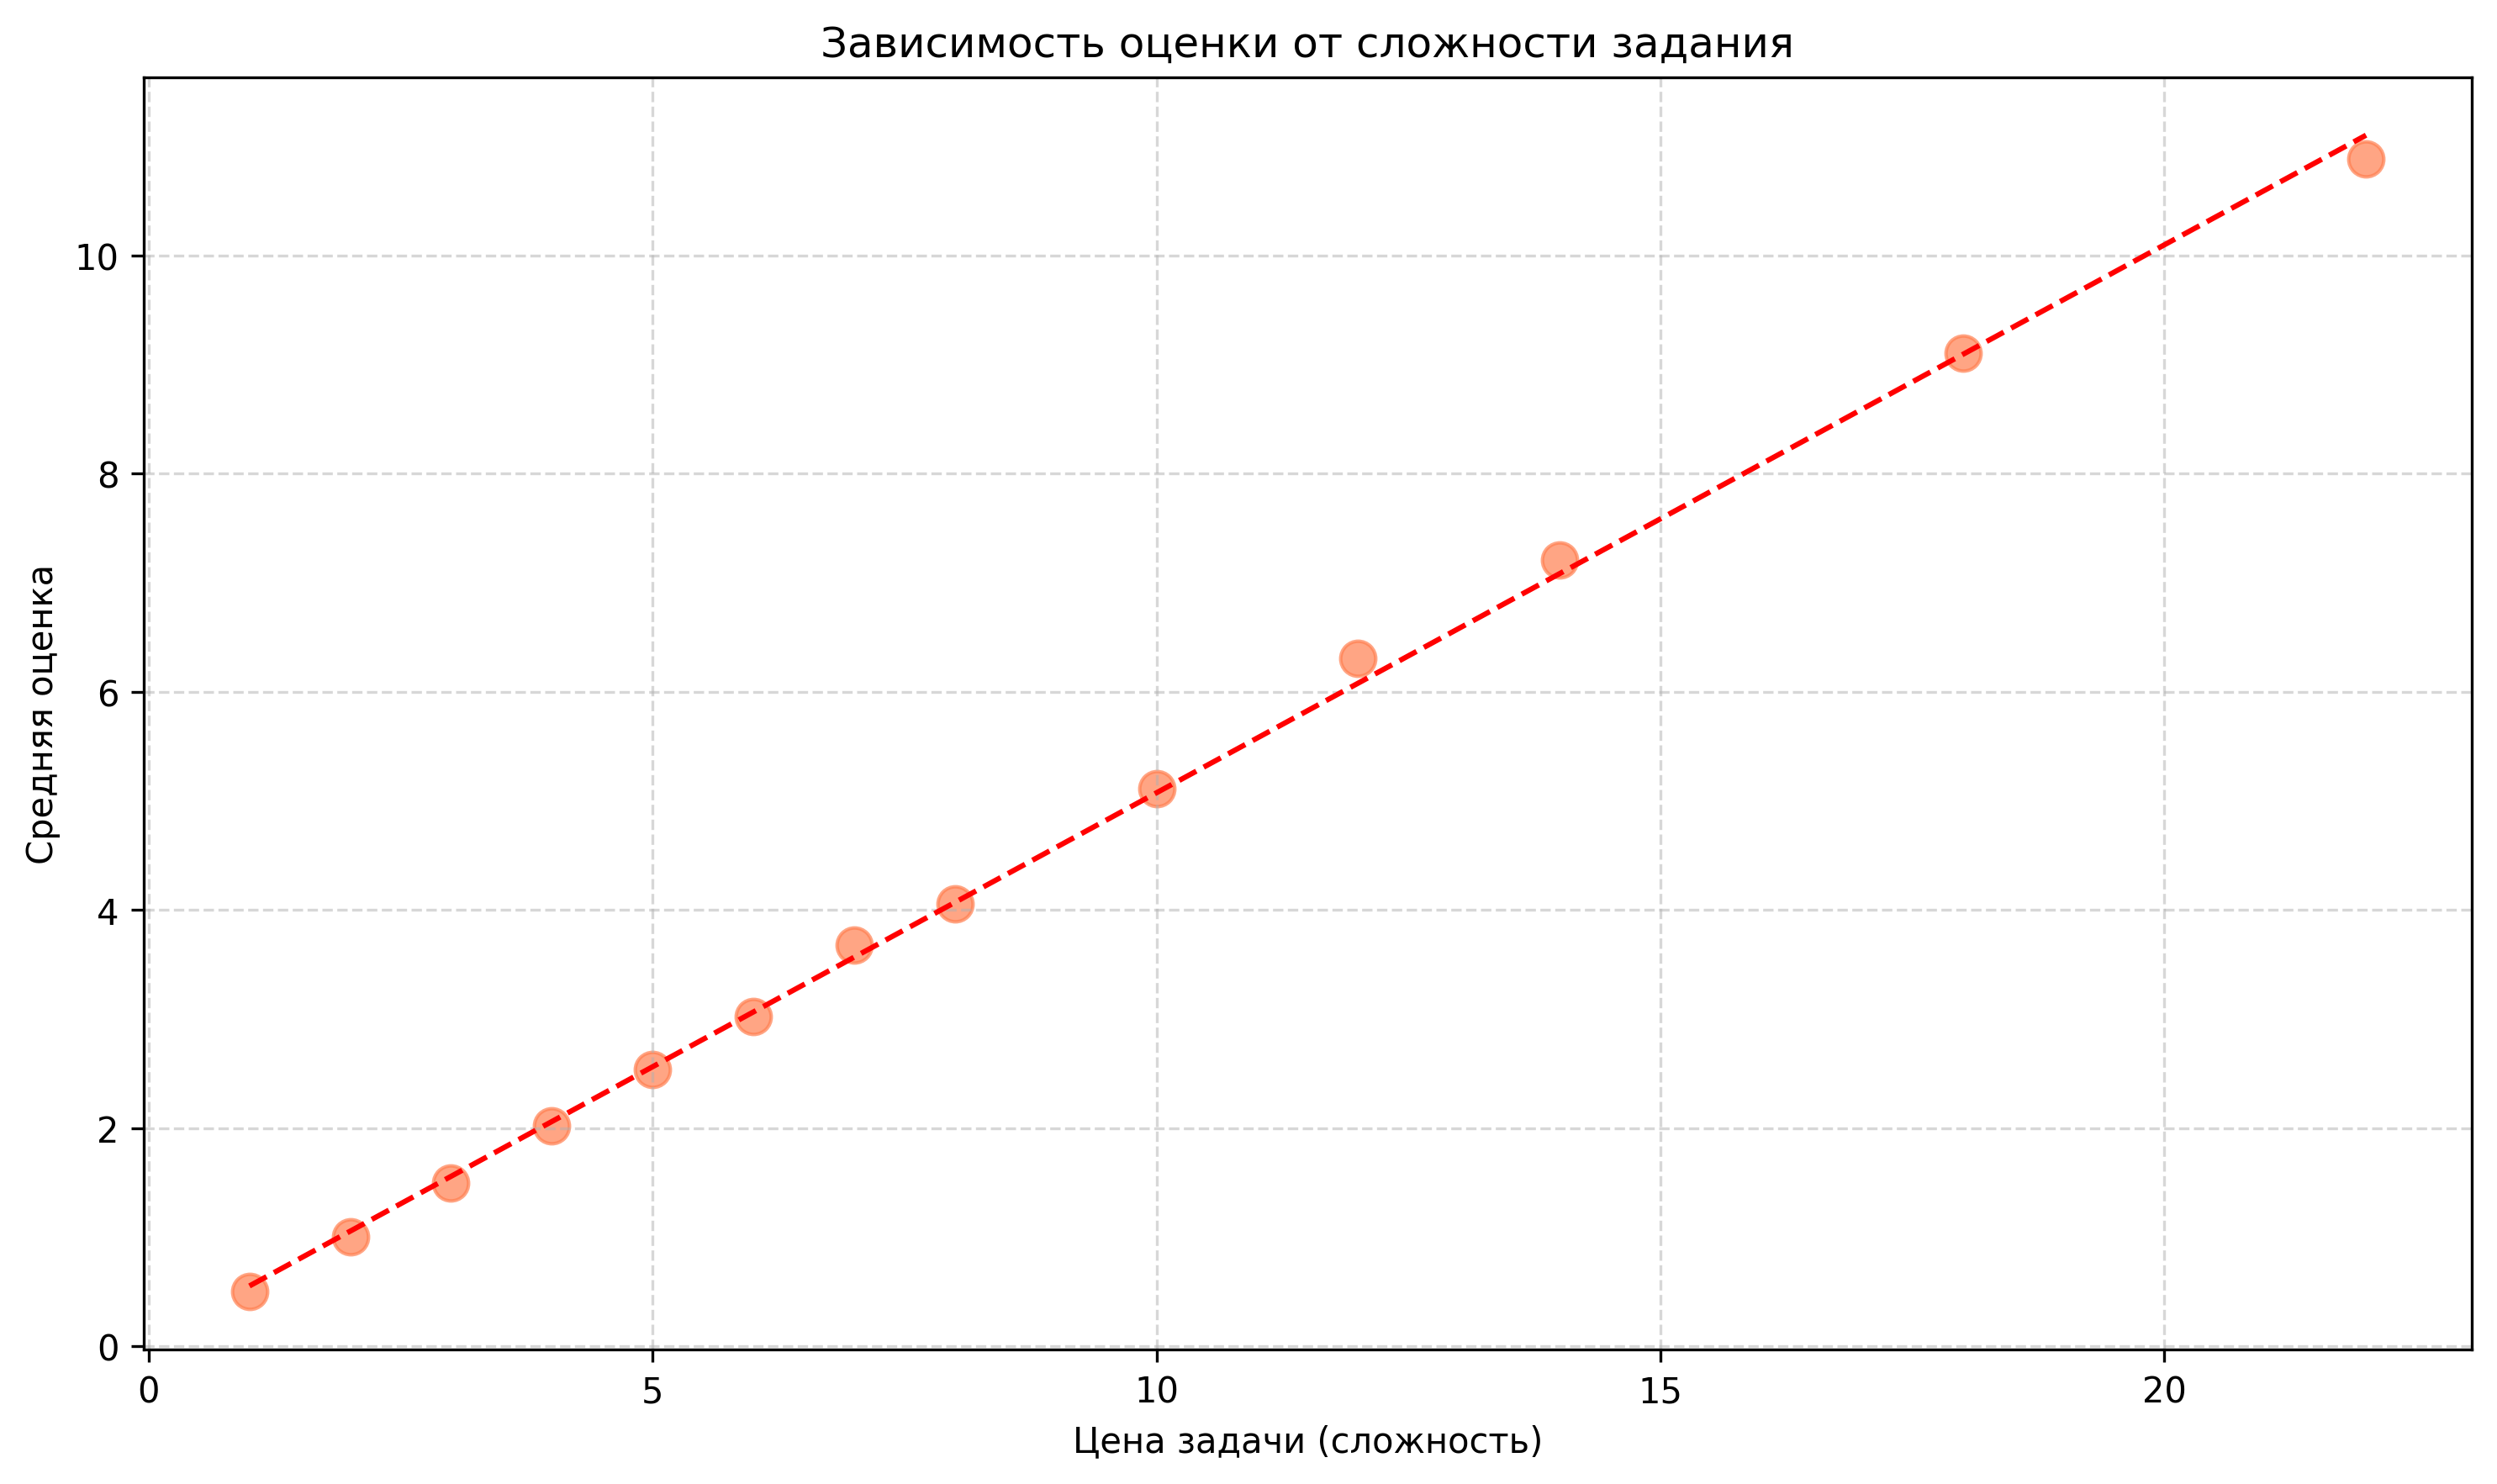
\includegraphics[width=14cm]{data/plots/task_price_vs_grade.png}
\newpage
\subsection{Отчет №2. Отчет о статусох экзаменов}
Выполнил: Колесников Михаил Леонидович.
Инструментальные средства: matplotlib, python.
Дата: 26.05.2025

\begin{lstlisting}[language=SQL, frame=none, numbers=none, caption={2. Круговая диаграмма статусов экзаменов}]
SELECT
    status,
    COUNT(*) AS count,
    ROUND(COUNT(*) * 100.0 / total.total, 2) AS percentage
FROM ExamResult
CROSS JOIN (SELECT COUNT(*) AS total FROM ExamResult) AS total
GROUP BY status, total.total;
            \end{lstlisting}
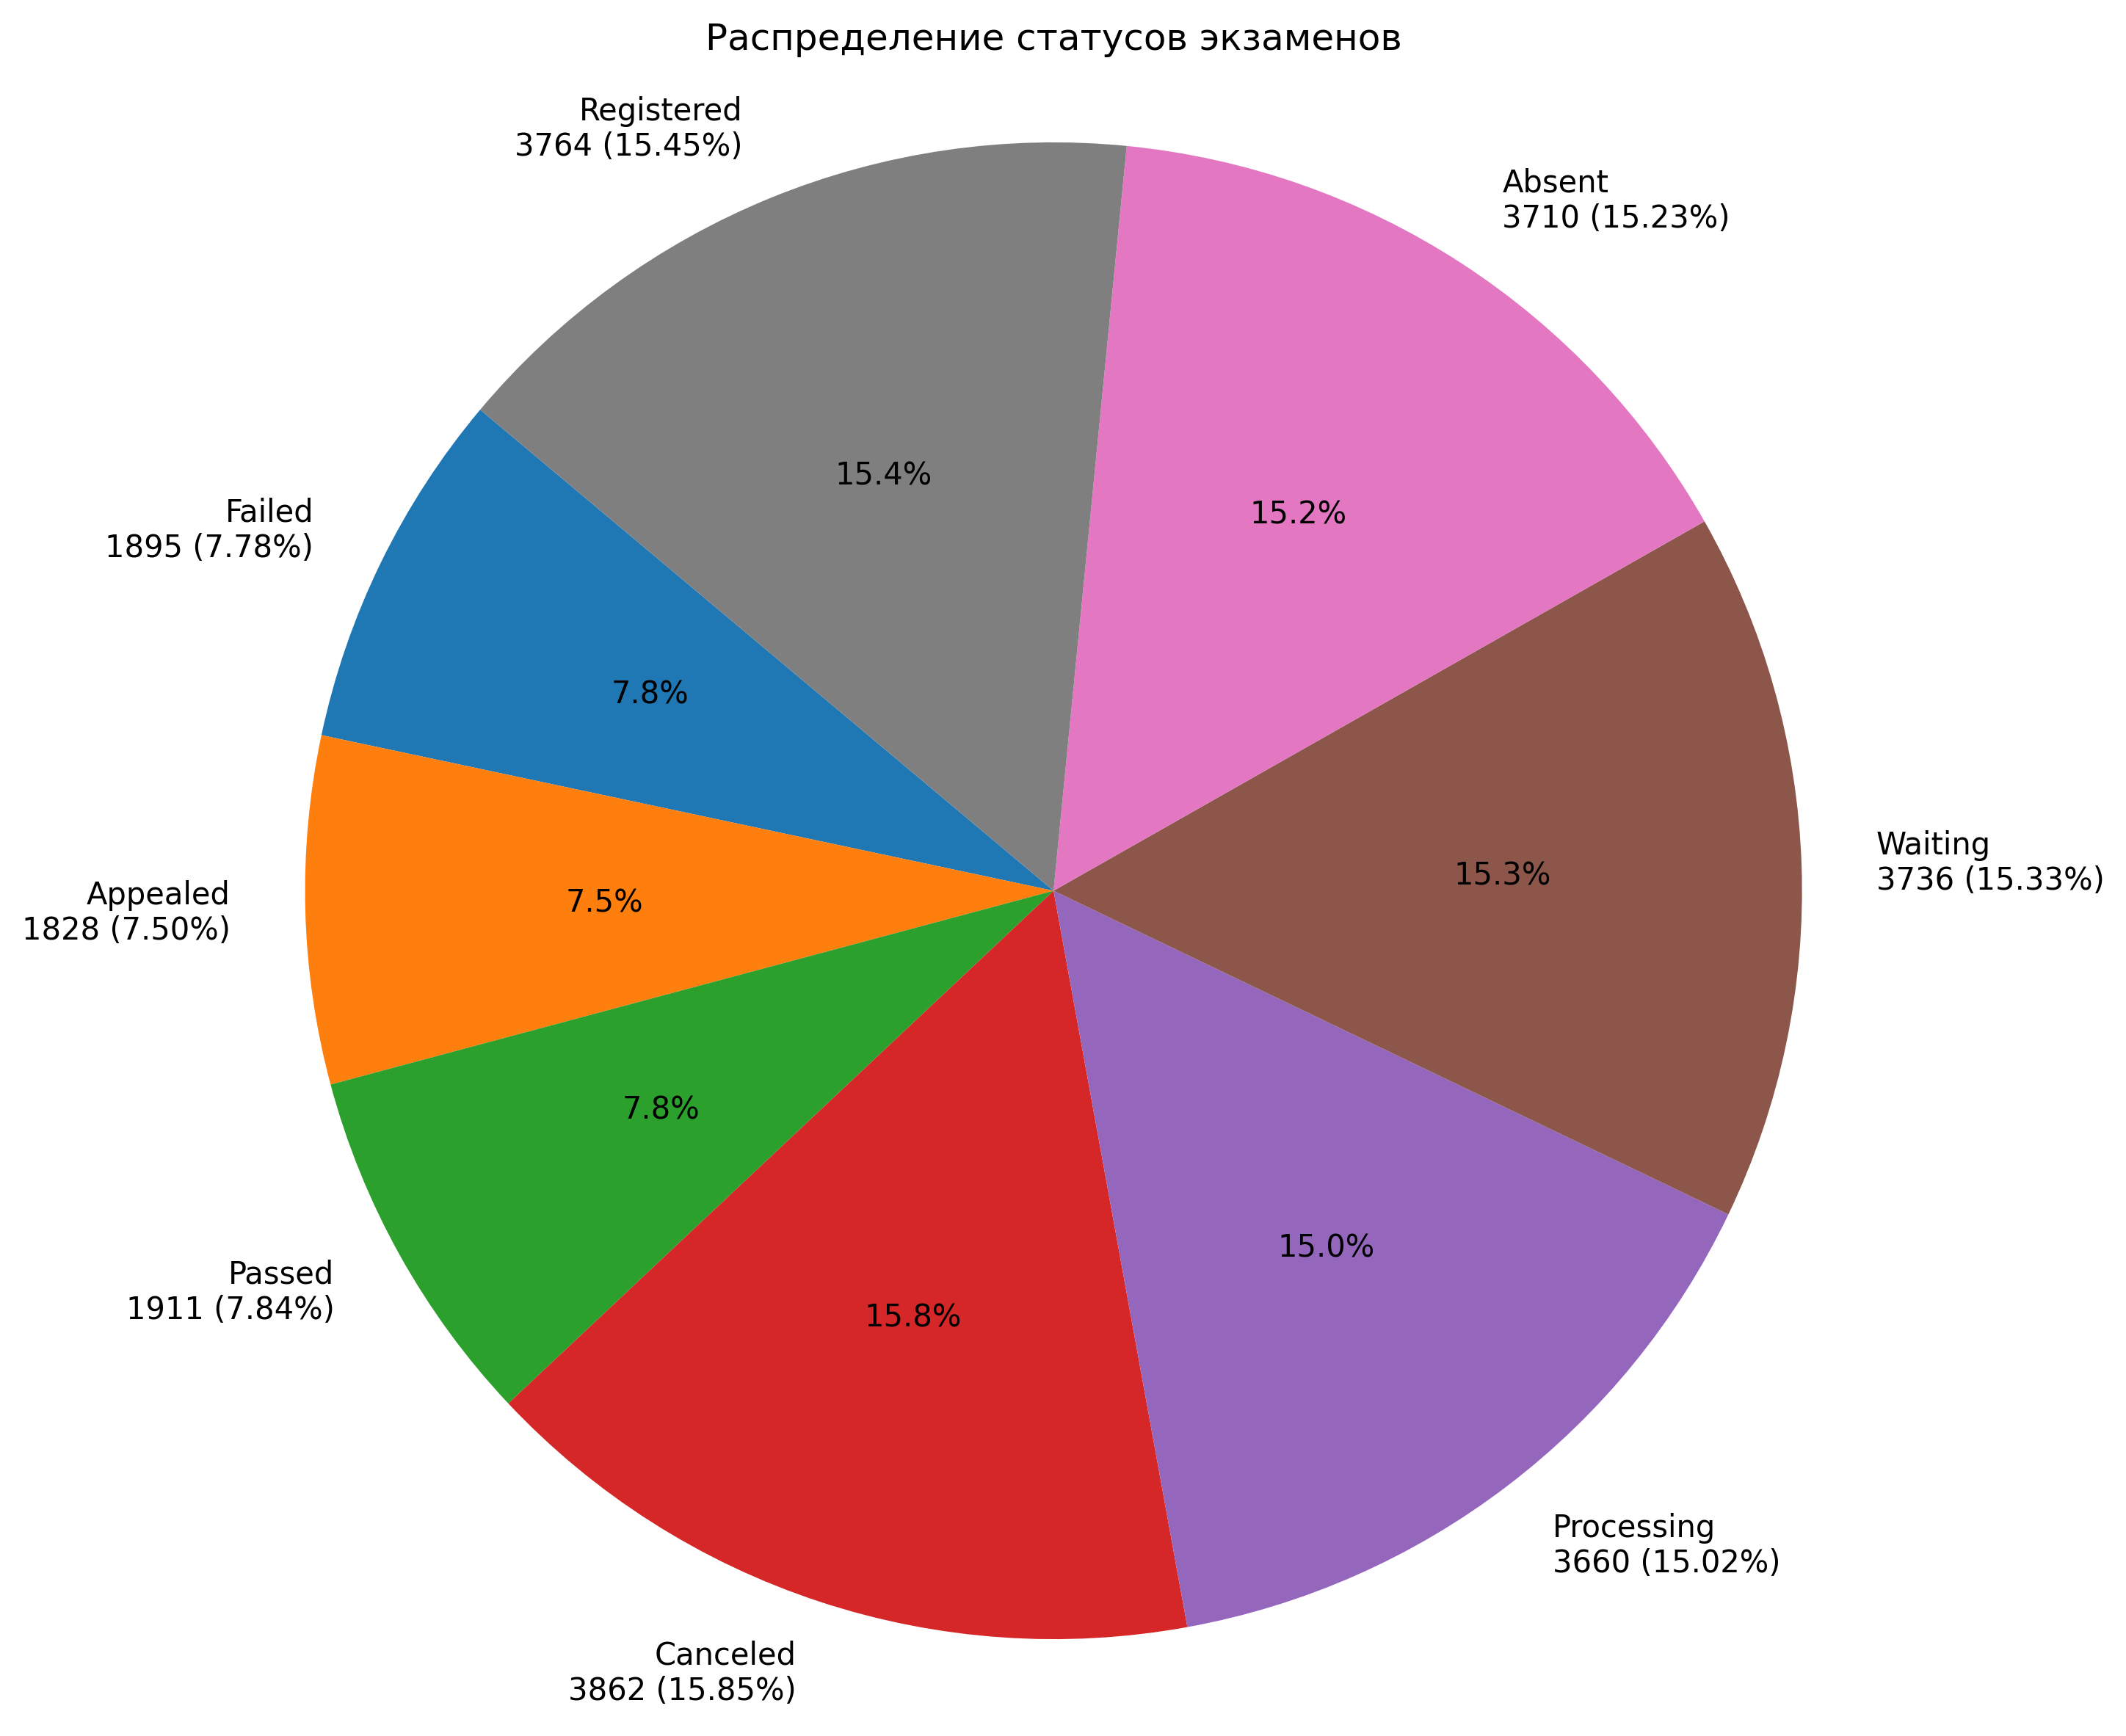
\includegraphics[width=14cm]{data/plots/exam_statuses_distribution.png}
\newpage
\subsection{Отчет №3. Отчет о распределении учащихся по школах}
Выполнил: Колесников Михаил Леонидович.
Инструментальные средства: matplotlib, python.
Дата: 26.05.2025

\begin{lstlisting}[language=SQL, frame=none, numbers=none, caption={3. Столбчатая диаграмма распределения учащихся по школам}]
SELECT s.school_name, COUNT(p.person_id) AS student_count
FROM School s
JOIN Person p ON s.school_id = p.school_id
WHERE p.role = 'SchoolChild'
GROUP BY s.school_name
ORDER BY student_count DESC;
            \end{lstlisting}
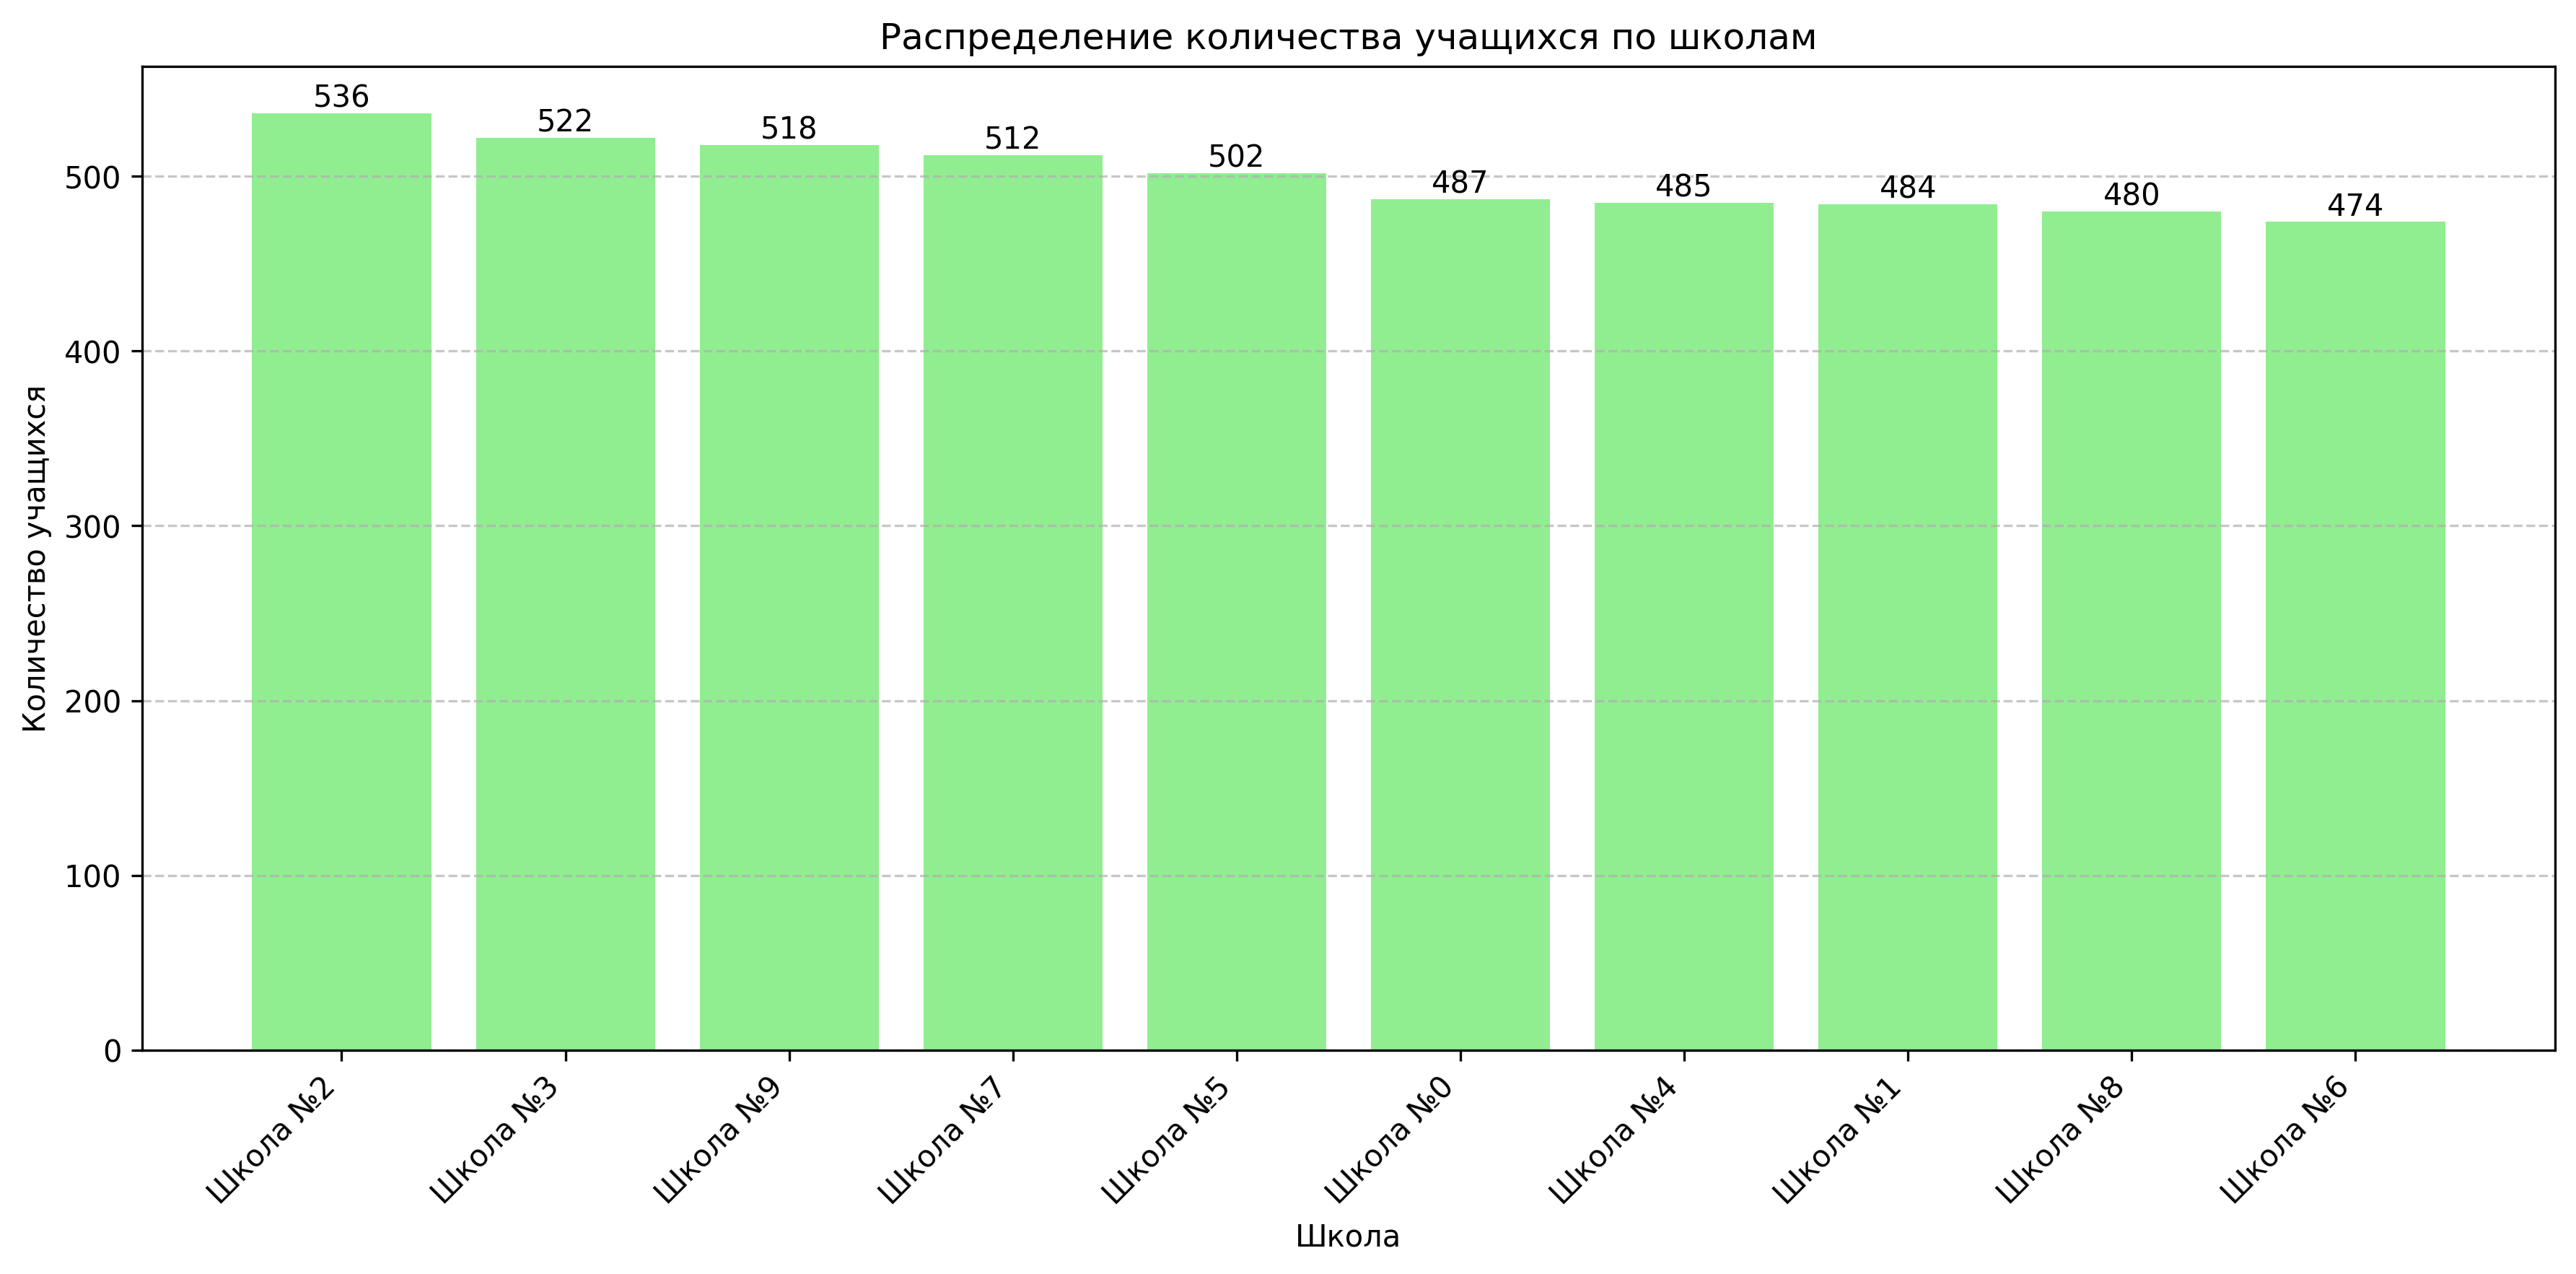
\includegraphics[width=14cm]{data/plots/students_per_school.png}
\newpage
\section{Приложение}
\section*{\hfill Приложение 1\hfill}
\subsection{Создание базы данных}
\label{subsec:db-create}
\lstinputlisting[language=yaml, label={lst:docker-compose}, caption={Конфигурация Docker Compose}, frame=none, numbers=none]{data/database_creating.yml}

\subsection{Создание таблиц}
\label{subsec:table-create}
\lstinputlisting[language=SQL, label={lst:sql-example}, caption={SQL-запросы для создания таблиц}, frame=none, numbers=none]{data/tables_creating.sql}

\section*{\hfill Приложение 2\hfill}
\subsection{Заполнение таблиц. ETL-процессы загрузки базы данных}

\subsubsection{}
\label{subsec:python1}
\lstinputlisting[language=python, label={lst:python1}, frame=none, numbers=none, caption={python-код для генерации заданий}]{/home/user_name/VScodeProjects/DB2/tables_filling/create_tasks.py}
\subsubsection{}
\label{subsec:python2}
\lstinputlisting[language=python, label={lst:python2}, frame=none, numbers=none, caption={python-код для генерации школ}]{/home/user_name/VScodeProjects/DB2/tables_filling/create_schools.py}
\subsubsection{}
\label{subsec:python3}
\lstinputlisting[language=python, label={lst:python3}, frame=none, numbers=none, caption={python-код для генерации экзаменов}]{/home/user_name/VScodeProjects/DB2/tables_filling/create_exams.py}
\subsubsection{}
\label{subsec:python4}
\lstinputlisting[language=python, label={lst:python4}, frame=none, numbers=none, caption={python-код для генерации учителей}]{/home/user_name/VScodeProjects/DB2/tables_filling/create_teachers.py}
\subsubsection{}
\label{subsec:python5}
\lstinputlisting[language=python, label={lst:python5}, frame=none, numbers=none, caption={python-код для генерации школьников}]{/home/user_name/VScodeProjects/DB2/tables_filling/create_schoolchildren.py}

\section*{\hfill Приложение 3\hfill}
\subsection{Запросы в терминах SQL}
\subsubsection{}
\label{subsec:sql1}
\begin{lstlisting}[language=SQL, label={lst:sql1}, frame=none, numbers=none, caption={SQL-запрос 1}]
SELECT DISTINCT p.person_id
FROM Person p
JOIN Subject s ON p.subject_id = s.subject_id
JOIN PersonExam pe ON p.person_id = pe.person_id
WHERE p.role = 'Teacher' AND s.name = 'Name';
            \end{lstlisting}
\subsubsection{}
\label{subsec:sql2}
\begin{lstlisting}[language=SQL, label={lst:sql2}, frame=none, numbers=none, caption={SQL-запрос 2}]
SELECT p.person_id
FROM Person p
WHERE p.role = 'SchoolChild' 
AND p.person_id NOT IN (SELECT person_id FROM PersonExam);
\end{lstlisting}
\subsubsection{}
\label{subsec:sql3}
\begin{lstlisting}[language=SQL, label={lst:sql3}, frame=none, numbers=none, caption={SQL-запрос 3}]
SELECT DISTINCT s.subject_id
FROM Exam e
JOIN Classroom c ON e.classroom_id = c.classroom_id
JOIN Subject s ON e.subject_id = s.subject_id
JOIN School sc ON c.school_id = sc.school_id
WHERE sc.school_name = 'Школа №0';
            \end{lstlisting}
\subsubsection{}
\label{subsec:sql4}
\begin{lstlisting}[language=SQL, label={lst:sql4}, frame=none, numbers=none, caption={SQL-запрос 4}]
SELECT DISTINCT p.person_id
FROM Person p
JOIN ExamResult er ON p.person_id = er.person_id
WHERE p.role = 'SchoolChild' AND er.score < 40;
            \end{lstlisting}
\subsubsection{}
\label{subsec:sql5}
\begin{lstlisting}[language=SQL, label={lst:sql5}, frame=none, numbers=none, caption={SQL-запрос 5}]
SELECT s.school_id
FROM School s
WHERE s.school_id NOT IN (SELECT school_id FROM Exam);
\end{lstlisting}
\subsubsection{}
\label{subsec:sql6}
\begin{lstlisting}[language=SQL, label={lst:sql6}, frame=none, numbers=none, caption={SQL-запрос 6}]
WITH SchoolChildren AS (
    SELECT p.person_id, er.score
    FROM Person p
    JOIN ExamResult er ON p.person_id = er.person_id
    WHERE p.role = 'SchoolChild'
)
SELECT DISTINCT person_id AS id
FROM SchoolChildren sc1
WHERE NOT EXISTS (
    SELECT 1 
    FROM SchoolChildren sc2 
    WHERE sc1.person_id = sc2.person_id AND sc2.score != 100
);
            \end{lstlisting}

\subsubsection{}
\label{subsec:sql7}
\begin{lstlisting}[language=SQL, label={lst:sql7}, frame=none, numbers=none, caption={SQL-запрос 7}]
SELECT 
    s.school_name,
    sub.name AS subject_name,
    COUNT(er.exam_result_id) AS exams_taken,
    AVG(er.score) AS avg_score,
    MAX(er.score) AS max_score
FROM 
    ExamResult er
    JOIN Subject sub ON er.subject_id = sub.subject_id
    JOIN Person p ON er.person_id = p.person_id
    JOIN School s ON p.school_id = s.school_id
GROUP BY 
    s.school_name, sub.name
HAVING 
    AVG(er.score) > 70 AND
    COUNT(er.exam_result_id) > 5
ORDER BY 
    avg_score DESC;
            \end{lstlisting}
\subsubsection{}
\label{subsec:sql8}
\begin{lstlisting}[language=SQL, label={lst:sql8}, frame=none, numbers=none, caption={SQL-запрос 8}]
WITH student_rank AS (
    SELECT 
        p.person_id,
        AVG(er.score) AS average_score,
        DENSE_RANK() OVER (ORDER BY AVG(er.score) DESC) AS rank
    FROM 
        Person p
        JOIN ExamResult er ON p.person_id = er.person_id
    WHERE 
        p.role = 'SchoolChild'
        AND er.status = 'Passed'
    GROUP BY 
        p.person_id
)
SELECT 
    person_id,
    ROUND(average_score, 2)
FROM 
    student_rank
WHERE 
    rank = 1;
            \end{lstlisting}


\end{document}